\documentclass[10pt]{article}
\usepackage{fancyhdr}
\usepackage{listings}
\usepackage{graphicx}
\usepackage[english]{babel}
\usepackage{multirow}

\setlength{\textwidth}{7.25in}
\setlength{\textheight}{9.0in}
\setlength{\topmargin}{-0.75in}
\setlength{\oddsidemargin}{-0.5in}
\setlength{\evensidemargin}{-0.5in}
\setlength{\headheight}{47pt}

\setlength\parindent{0pt}

\fancyhead[R]{CS 111C Jessica Masters\\
				Homework 11\\
				Chapters 30-31 Graphs\\
				Richard Szeto}
				
\pagestyle{fancy}

\lstset{language=Java}

\begin{document}

\begin{center}
	\Large{\textbf{Homework 11: Graphs}}
\end{center}

\section{Chapter 29: Balanced Search Trees}
\begin{enumerate}
	\item[3.] Add 62 and 65 to the 2-3 tree in Figure 29-27b
		\begin{itemize}
			\item Show the final resulting tree
		\end{itemize}
		
		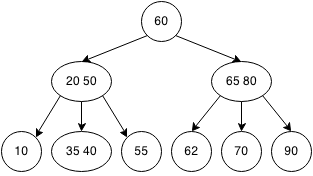
\includegraphics[scale=0.5]{images/29_3.png}
	
	\item[4.] Add 62 and 65 to the 2-4 tree in Figure 29-27c
		\begin{itemize}
			\item Show the final resulting tree
		\end{itemize}
		
		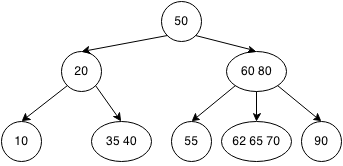
\includegraphics[scale=0.5]{images/29_4.png}
	
	\item[8.] What tree results when you add the values 10, 20, 30, 40, 50, 60, 70, 80, 90, and 100 to each of the following initially empty tree?
		\begin{itemize}
			\item Show what the tree looks like after \textbf{each} element is inserted. You do not need to show the "splitting" steps, but show what the tree looks like after each insertion. (There should be 10 trees shown for 8b and 10 for 8c).
		\end{itemize}
		\begin{enumerate}
			\item[(b)] A 2-3 tree
				\begin{enumerate}
					\item add 10
					
						
\includegraphics[scale=0.5]{images/29_8b_add10.png}
					\item add 20
					
						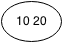
\includegraphics[scale=0.5]{images/29_8b_add20.png}
					\item add 30
					
						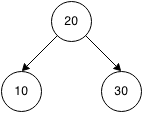
\includegraphics[scale=0.5]{images/29_8b_add30.png}
					\item add 40
					
						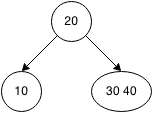
\includegraphics[scale=0.5]{images/29_8b_add40.png}
					\item add 50
						
						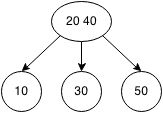
\includegraphics[scale=0.5]{images/29_8b_add50.png}
					\item add 60
						
						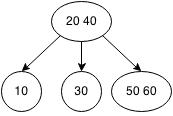
\includegraphics[scale=0.5]{images/29_8b_add60.png}
					\item add 70
					
						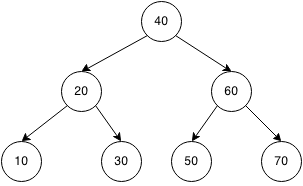
\includegraphics[scale=0.5]{images/29_8b_add70.png}
					\item add 80
						
						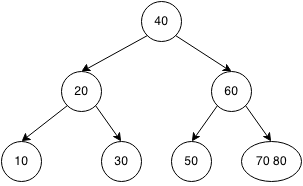
\includegraphics[scale=0.5]{images/29_8b_add80.png}
					\item add 90
						
						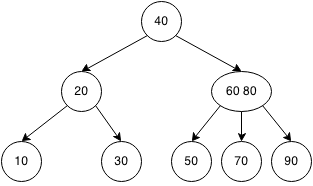
\includegraphics[scale=0.5]{images/29_8b_add90.png}
					\item add 100
						
						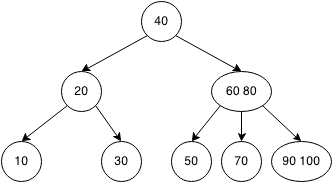
\includegraphics[scale=0.5]{images/29_8b_add100.png}
				\end{enumerate}
			
			\item[(c)] A 2-4 tree
				\begin{enumerate}
					\item add 10
					
						
\includegraphics[scale=0.5]{images/29_8c_add10.png}
					\item add 20
					
						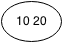
\includegraphics[scale=0.5]{images/29_8c_add20.png}
					\item add 30
					
						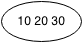
\includegraphics[scale=0.5]{images/29_8c_add30.png}
					\item add 40
					
						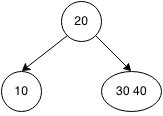
\includegraphics[scale=0.5]{images/29_8c_add40.png}
					\item add 50
					
						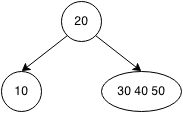
\includegraphics[scale=0.5]{images/29_8c_add50.png}
					\item add 60
					
						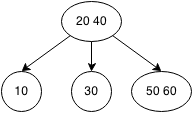
\includegraphics[scale=0.5]{images/29_8c_add60.png}
					\item add 70
					
						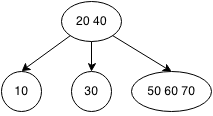
\includegraphics[scale=0.5]{images/29_8c_add70.png}
					\item add 80
					
						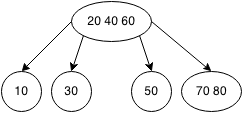
\includegraphics[scale=0.5]{images/29_8c_add80.png}
					\item add 90
					
						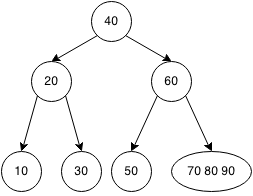
\includegraphics[scale=0.5]{images/29_8c_add90.png}
					\item add 100
					
						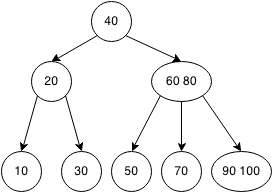
\includegraphics[scale=0.5]{images/29_8c_add100.png}
				\end{enumerate}
		\end{enumerate}
\end{enumerate}

\section{Chapter 30: Graphs}
\begin{enumerate}
	\item[2.] Describe each graph in Figure 30-22, using the terms introduced in Segments 30.1 through 30.4.
		\begin{itemize}
			\item Describe the following for each graph:
				\begin{itemize}
					\item directed/undirected
					\item number of nodes
					\item number of edges
					\item unweighted/weighted
					\item connected/disconnected
					\item complete/not complete
					\item cyclic/acyclic
				\end{itemize}
		\end{itemize}
		
		\begin{enumerate}
			\item ~
				\begin{itemize}
					\item undirected
					\item 5 vertices
					\item 4 edges
					\item unweighted
					\item disconnected
					\item not complete
					\item cyclic
				\end{itemize}
			\item ~
				\begin{itemize}
					\item undirected
					\item 5 vertices
					\item 8 edges
					\item unweighted
					\item connected
					\item not complete
					\item cyclic
				\end{itemize}
			\item ~
				\begin{itemize}
					\item undirected
					\item 4 vertices
					\item 5 edges
					\item unweighted
					\item connected
					\item not complete
					\item cyclic
				\end{itemize}
		\end{enumerate}
	
	\item[4.] In what order does a breadth-first traversal visit the vertices in the graph in Figure 30-10 when you begin at
		\begin{enumerate}
			\item Vertex G
				
				\vspace{0.5cm}
				My choice for traversal order was based on alphabetical order.\\
				GHIFCBE
				\vspace{0.5cm}
				
			\item Vertex F
				
				\vspace{0.5cm}
				My choice for traversal order was based on alphabetical order.\\
				FCHBIE
				\vspace{0.5cm}
				
		\end{enumerate}
	
	\item[5.] Repeat the previous exercise, but perform a depth-first traversal instead.
		\begin{enumerate}
			\item Vertex G
				
				\vspace{0.5cm}
				My choice for traversal order was based on alphabetical order.\\
				GHIFCBE
				\vspace{0.5cm}
			\item Vertex F
				
				\vspace{0.5cm}
				My choice for traversal order was based on alphabetical order.\\
				FCBEHI
				\vspace{0.5cm}
		\end{enumerate}
	
	\item[6.] Consider the directed graph that appears in Figure 30-10, and remove the edge between vertices E and F, and the edge between vertices F and H.
		\begin{enumerate}
			\item In what order will a breadth-first traversal visit the vertices when you begin at vertex A?
			
				\vspace{0.5cm}
				My choice for traversal order was based on alphabetical order.\\
				ABDEGHIFC
				\vspace{0.5cm}
				
			\item Repeat part \textit{a}, but perform a depth-first traversal instead.
				
				\vspace{0.5cm}
				My choice for traversal order was based on alphabetical order.\\
				ABEHIFCDG
				\vspace{0.5cm}
				
		\end{enumerate}
	
	\item[8.] Construct the topological ordering for the weighted, directed, acyclic graph in Figure 30-23.
		
		\vspace{0.5cm}
		AFBCDEMLJKHGI
		\vspace{0.5cm}
	
	\item[11.] A tree is a connected graph without cycles.
		\begin{enumerate}
			\item What is the smallest number of edges that could be removed from the graph in Figure 30-1 to make it a tree?
				
				\vspace{0.5cm}
				Only 1 edge needs to be removed.
				\vspace{0.5cm}
				
			\item Give one example of such a set of edges.
			
				\vspace{0.5cm}
				One example is to remove the edge connecting Orleans and Chatham.
				\vspace{0.5cm}
		\end{enumerate}
	
	\item[16.] Find a map of the routes of a major U.S. airline. Such maps are usually printed at the back of in-flight magazines. You could also search the Internet for one. The map is a graph like the one in Figure 30-6. Consider the following pairs of cities:
		\begin{itemize}
			\item Providence (RI) and San Diego (CA)
			\item Albany (NY) and Phoenix (AZ)
			\item Boston (MA) and Baltimore (MD)
			\item Dallas (TX) and Detroit (MI)
			\item Charlotte (NC) and Chicago (IL)
			\item Portland (ME) and Portland (OR)		
		\end{itemize}
		
		\begin{itemize}
			\item I recommend using the interactive map on the Jet Blue website: http://www.jetblue.com/WhereWeJet/. If you use this, use Buffalo, NY instead of Albany, NY. If you use a different airline, you must include the map or the URL in your answer.
		\end{itemize}
		
		\begin{enumerate}
			\item Which pairs of cities in this list have edges (nonstop flights) between them?
				\begin{itemize}
					\item Boston (MA) and Baltimore (MD)
				\end{itemize}
			\item Which pairs are not connected by any path?
				\begin{itemize}
					\item Providence (RI) and San Diego (CA)
				\end{itemize}
			
			\item For each of the remaining pairs, find the path with the fewest edges.
				\begin{itemize}
					\item Buffalo (NY) and Phoenix (AZ) have 2 edges
						\begin{itemize}
							\item Buffalo (NY) and Boston (MA)
							\item Boston (MA) AND Phoenix (AZ)
						\end{itemize}
						
						\vspace{0.5cm}
						\begin{itemize}
							\item Buffalo (NY) and New York City (NY)
							\item New York City (NY) and Phoenix (AZ)
						\end{itemize}
					\item Dallas (TX) and Detroit (MI) have 2 edges
						\begin{itemize}
							\item Dalls (TX) and Boston (MA)
							\item Boston (MA) and Detroit (MI)
						\end{itemize}
					\item Charlotte (NC) and Chicago (IL) have 2 edges
						\begin{itemize}
							\item Charlotte (NC) and New York City (NY)
							\item New York City (NY) and Chicago (IL)
						\end{itemize}
					\item Portland (ME) and Portland (OR) have 2 edges
						\begin{itemize}
							\item Portland (ME) and New York City (NY)
							\item New York City (NY) and Portland (OR)
						\end{itemize}
				\end{itemize}
		\end{enumerate}
	
	\item[EC.] Describe real-world situations that could be represented by a graph with the properties below. For each graph, describe what the nodes are and what an edge represents.
		\begin{itemize}
			\item directed and disconnected
			
				\vspace{0.5cm}
				Offered routes of airlines can be directed and disconnected. An offered path from one city to another may be different when the source and destination vertices are reversed, so the graph is directed. There may be offered paths to fly in a small area in the world that do not have an offered path to anywhere else in the world, so the graph will be disconnected.
				\vspace{0.5cm}
				
			\item undirected and disconnected
				
				\vspace{0.5cm}
				Friends lists on Facebook all over the world. Each friend that a person has on Facebook must be mutual between the two parties, so the edges are undirected. There may be a group of friends that are only friends with each other, and nobody else. Thus the graph is disconnected.
				\vspace{0.5cm}
				
			\item complete
				
				\vspace{0.5cm}
				The social relationship between a happy household. There are households where everyone in the household love each other, including themselves. This would create a complete graph.
				\vspace{0.5cm}
		\end{itemize}
\end{enumerate}

\section{Chapter 31: Graph Implementations}
\begin{enumerate}
	\item[1.] What adjacency matrix represents the graph in Figure 30-15a of the previous chapter?
	
		\begin{tabular}{ r|c|c|c|c|c|c|c|c|c| }
			\multicolumn{1}{r}{} & \multicolumn{1}{c}{A} & \multicolumn{1}{c}{B} & \multicolumn{1}{c}{C} & \multicolumn{1}{c}{D} & \multicolumn{1}{c}{E} & \multicolumn{1}{c}{F} & \multicolumn{1}{c}{G} & \multicolumn{1}{c}{H} & \multicolumn{1}{c}{I} \\
			
			\cline{2-10}
			
			\multicolumn{1}{r}{\multirow{2}{*}{A}} & \multicolumn{1}{ |c| }{\multirow{2}{*}{}} & \multicolumn{1}{ |c| }{\multirow{2}{*}{T}} & \multicolumn{1}{ |c| }{\multirow{2}{*}{}} & \multicolumn{1}{ |c| }{\multirow{2}{*}{T}} & \multicolumn{1}{ |c| }{\multirow{2}{*}{T}} & \multicolumn{1}{ |c| }{\multirow{2}{*}{}} & \multicolumn{1}{ |c| }{\multirow{2}{*}{}} & \multicolumn{1}{ |c| }{\multirow{2}{*}{}} & \multicolumn{1}{ |c| }{\multirow{2}{*}{}} \\
			\multicolumn{1}{r}{} & \multicolumn{1}{ |c| }{} & \multicolumn{1}{ |c| }{} & \multicolumn{1}{ |c| }{} & \multicolumn{1}{ |c| }{} & \multicolumn{1}{ |c| }{} & \multicolumn{1}{ |c| }{} & \multicolumn{1}{ |c| }{} & \multicolumn{1}{ |c| }{} & \multicolumn{1}{ |c| }{} \\
			
			\cline{2-10}
			
			\multicolumn{1}{r}{\multirow{2}{*}{B}} & \multicolumn{1}{ |c| }{\multirow{2}{*}{}} & \multicolumn{1}{ |c| }{\multirow{2}{*}{}} & \multicolumn{1}{ |c| }{\multirow{2}{*}{}} & \multicolumn{1}{ |c| }{\multirow{2}{*}{}} & \multicolumn{1}{ |c| }{\multirow{2}{*}{T}} & \multicolumn{1}{ |c| }{\multirow{2}{*}{}} & \multicolumn{1}{ |c| }{\multirow{2}{*}{}} & \multicolumn{1}{ |c| }{\multirow{2}{*}{}} & \multicolumn{1}{ |c| }{\multirow{2}{*}{}} \\
			\multicolumn{1}{r}{} & \multicolumn{1}{ |c| }{} & \multicolumn{1}{ |c| }{} & \multicolumn{1}{ |c| }{} & \multicolumn{1}{ |c| }{} & \multicolumn{1}{ |c| }{} & \multicolumn{1}{ |c| }{} & \multicolumn{1}{ |c| }{} & \multicolumn{1}{ |c| }{} & \multicolumn{1}{ |c| }{} \\
			
			\cline{2-10}
			
			\multicolumn{1}{r}{\multirow{2}{*}{C}} & \multicolumn{1}{ |c| }{\multirow{2}{*}{}} & \multicolumn{1}{ |c| }{\multirow{2}{*}{T}} & \multicolumn{1}{ |c| }{\multirow{2}{*}{}} & \multicolumn{1}{ |c| }{\multirow{2}{*}{}} & \multicolumn{1}{ |c| }{\multirow{2}{*}{}} & \multicolumn{1}{ |c| }{\multirow{2}{*}{}} & \multicolumn{1}{ |c| }{\multirow{2}{*}{}} & \multicolumn{1}{ |c| }{\multirow{2}{*}{}} & \multicolumn{1}{ |c| }{\multirow{2}{*}{}} \\
			\multicolumn{1}{r}{} & \multicolumn{1}{ |c| }{} & \multicolumn{1}{ |c| }{} & \multicolumn{1}{ |c| }{} & \multicolumn{1}{ |c| }{} & \multicolumn{1}{ |c| }{} & \multicolumn{1}{ |c| }{} & \multicolumn{1}{ |c| }{} & \multicolumn{1}{ |c| }{} & \multicolumn{1}{ |c| }{} \\
			
			\cline{2-10}
			
			\multicolumn{1}{r}{\multirow{2}{*}{D}} & \multicolumn{1}{ |c| }{\multirow{2}{*}{}} & \multicolumn{1}{ |c| }{\multirow{2}{*}{}} & \multicolumn{1}{ |c| }{\multirow{2}{*}{}} & \multicolumn{1}{ |c| }{\multirow{2}{*}{}} & \multicolumn{1}{ |c| }{\multirow{2}{*}{}} & \multicolumn{1}{ |c| }{\multirow{2}{*}{}} & \multicolumn{1}{ |c| }{\multirow{2}{*}{T}} & \multicolumn{1}{ |c| }{\multirow{2}{*}{}} & \multicolumn{1}{ |c| }{\multirow{2}{*}{}} \\
			\multicolumn{1}{r}{} & \multicolumn{1}{ |c| }{} & \multicolumn{1}{ |c| }{} & \multicolumn{1}{ |c| }{} & \multicolumn{1}{ |c| }{} & \multicolumn{1}{ |c| }{} & \multicolumn{1}{ |c| }{} & \multicolumn{1}{ |c| }{} & \multicolumn{1}{ |c| }{} & \multicolumn{1}{ |c| }{} \\
			
			\cline{2-10}
			
			\multicolumn{1}{r}{\multirow{2}{*}{E}} & \multicolumn{1}{ |c| }{\multirow{2}{*}{}} & \multicolumn{1}{ |c| }{\multirow{2}{*}{}} & \multicolumn{1}{ |c| }{\multirow{2}{*}{}} & \multicolumn{1}{ |c| }{\multirow{2}{*}{}} & \multicolumn{1}{ |c| }{\multirow{2}{*}{}} & \multicolumn{1}{ |c| }{\multirow{2}{*}{T}} & \multicolumn{1}{ |c| }{\multirow{2}{*}{}} & \multicolumn{1}{ |c| }{\multirow{2}{*}{T}} & \multicolumn{1}{ |c| }{\multirow{2}{*}{}} \\
			\multicolumn{1}{r}{} & \multicolumn{1}{ |c| }{} & \multicolumn{1}{ |c| }{} & \multicolumn{1}{ |c| }{} & \multicolumn{1}{ |c| }{} & \multicolumn{1}{ |c| }{} & \multicolumn{1}{ |c| }{} & \multicolumn{1}{ |c| }{} & \multicolumn{1}{ |c| }{} & \multicolumn{1}{ |c| }{} \\
			
			\cline{2-10}
			
			\multicolumn{1}{r}{\multirow{2}{*}{F}} & \multicolumn{1}{ |c| }{\multirow{2}{*}{}} & \multicolumn{1}{ |c| }{\multirow{2}{*}{}} & \multicolumn{1}{ |c| }{\multirow{2}{*}{T}} & \multicolumn{1}{ |c| }{\multirow{2}{*}{}} & \multicolumn{1}{ |c| }{\multirow{2}{*}{}} & \multicolumn{1}{ |c| }{\multirow{2}{*}{}} & \multicolumn{1}{ |c| }{\multirow{2}{*}{}} & \multicolumn{1}{ |c| }{\multirow{2}{*}{T}} & \multicolumn{1}{ |c| }{\multirow{2}{*}{}} \\
			\multicolumn{1}{r}{} & \multicolumn{1}{ |c| }{} & \multicolumn{1}{ |c| }{} & \multicolumn{1}{ |c| }{} & \multicolumn{1}{ |c| }{} & \multicolumn{1}{ |c| }{} & \multicolumn{1}{ |c| }{} & \multicolumn{1}{ |c| }{} & \multicolumn{1}{ |c| }{} & \multicolumn{1}{ |c| }{} \\
			
			\cline{2-10}
			
			\multicolumn{1}{r}{\multirow{2}{*}{G}} & \multicolumn{1}{ |c| }{\multirow{2}{*}{}} & \multicolumn{1}{ |c| }{\multirow{2}{*}{}} & \multicolumn{1}{ |c| }{\multirow{2}{*}{}} & \multicolumn{1}{ |c| }{\multirow{2}{*}{}} & \multicolumn{1}{ |c| }{\multirow{2}{*}{}} & \multicolumn{1}{ |c| }{\multirow{2}{*}{}} & \multicolumn{1}{ |c| }{\multirow{2}{*}{}} & \multicolumn{1}{ |c| }{\multirow{2}{*}{T}} & \multicolumn{1}{ |c| }{\multirow{2}{*}{}} \\
			\multicolumn{1}{r}{} & \multicolumn{1}{ |c| }{} & \multicolumn{1}{ |c| }{} & \multicolumn{1}{ |c| }{} & \multicolumn{1}{ |c| }{} & \multicolumn{1}{ |c| }{} & \multicolumn{1}{ |c| }{} & \multicolumn{1}{ |c| }{} & \multicolumn{1}{ |c| }{} & \multicolumn{1}{ |c| }{} \\
			
			\cline{2-10}
			
			\multicolumn{1}{r}{\multirow{2}{*}{H}} & \multicolumn{1}{ |c| }{\multirow{2}{*}{}} & \multicolumn{1}{ |c| }{\multirow{2}{*}{}} & \multicolumn{1}{ |c| }{\multirow{2}{*}{}} & \multicolumn{1}{ |c| }{\multirow{2}{*}{}} & \multicolumn{1}{ |c| }{\multirow{2}{*}{}} & \multicolumn{1}{ |c| }{\multirow{2}{*}{}} & \multicolumn{1}{ |c| }{\multirow{2}{*}{}} & \multicolumn{1}{ |c| }{\multirow{2}{*}{}} & \multicolumn{1}{ |c| }{\multirow{2}{*}{T}} \\
			\multicolumn{1}{r}{} & \multicolumn{1}{ |c| }{} & \multicolumn{1}{ |c| }{} & \multicolumn{1}{ |c| }{} & \multicolumn{1}{ |c| }{} & \multicolumn{1}{ |c| }{} & \multicolumn{1}{ |c| }{} & \multicolumn{1}{ |c| }{} & \multicolumn{1}{ |c| }{} & \multicolumn{1}{ |c| }{} \\
			
			\cline{2-10}
			
			\multicolumn{1}{r}{\multirow{2}{*}{I}} & \multicolumn{1}{ |c| }{\multirow{2}{*}{}} & \multicolumn{1}{ |c| }{\multirow{2}{*}{}} & \multicolumn{1}{ |c| }{\multirow{2}{*}{}} & \multicolumn{1}{ |c| }{\multirow{2}{*}{}} & \multicolumn{1}{ |c| }{\multirow{2}{*}{}} & \multicolumn{1}{ |c| }{\multirow{2}{*}{T}} & \multicolumn{1}{ |c| }{\multirow{2}{*}{}} & \multicolumn{1}{ |c| }{\multirow{2}{*}{}} & \multicolumn{1}{ |c| }{\multirow{2}{*}{}} \\
			\multicolumn{1}{r}{} & \multicolumn{1}{ |c| }{} & \multicolumn{1}{ |c| }{} & \multicolumn{1}{ |c| }{} & \multicolumn{1}{ |c| }{} & \multicolumn{1}{ |c| }{} & \multicolumn{1}{ |c| }{} & \multicolumn{1}{ |c| }{} & \multicolumn{1}{ |c| }{} & \multicolumn{1}{ |c| }{} \\
			
			\cline{2-10}
		
		\end{tabular}
	
	\item[2.] What adjacency matrix represents the graph in Figure 30-18a of the previous chapter?
	
		\begin{tabular}{ r|c|c|c|c|c|c|c|c|c| }
			\multicolumn{1}{r}{} & \multicolumn{1}{c}{A} & \multicolumn{1}{c}{B} & \multicolumn{1}{c}{C} & \multicolumn{1}{c}{D} & \multicolumn{1}{c}{E} & \multicolumn{1}{c}{F} & \multicolumn{1}{c}{G} & \multicolumn{1}{c}{H} & \multicolumn{1}{c}{I} \\
			
			\cline{2-10}
			
			\multicolumn{1}{r}{\multirow{2}{*}{A}} & \multicolumn{1}{ |c| }{\multirow{2}{*}{}} & \multicolumn{1}{ |c| }{\multirow{2}{*}{2}} & \multicolumn{1}{ |c| }{\multirow{2}{*}{}} & \multicolumn{1}{ |c| }{\multirow{2}{*}{5}} & \multicolumn{1}{ |c| }{\multirow{2}{*}{4}} & \multicolumn{1}{ |c| }{\multirow{2}{*}{}} & \multicolumn{1}{ |c| }{\multirow{2}{*}{}} & \multicolumn{1}{ |c| }{\multirow{2}{*}{}} & \multicolumn{1}{ |c| }{\multirow{2}{*}{}} \\
			\multicolumn{1}{r}{} & \multicolumn{1}{ |c| }{} & \multicolumn{1}{ |c| }{} & \multicolumn{1}{ |c| }{} & \multicolumn{1}{ |c| }{} & \multicolumn{1}{ |c| }{} & \multicolumn{1}{ |c| }{} & \multicolumn{1}{ |c| }{} & \multicolumn{1}{ |c| }{} & \multicolumn{1}{ |c| }{} \\
			
			\cline{2-10}
			
			\multicolumn{1}{r}{\multirow{2}{*}{B}} & \multicolumn{1}{ |c| }{\multirow{2}{*}{}} & \multicolumn{1}{ |c| }{\multirow{2}{*}{}} & \multicolumn{1}{ |c| }{\multirow{2}{*}{}} & \multicolumn{1}{ |c| }{\multirow{2}{*}{}} & \multicolumn{1}{ |c| }{\multirow{2}{*}{1}} & \multicolumn{1}{ |c| }{\multirow{2}{*}{}} & \multicolumn{1}{ |c| }{\multirow{2}{*}{}} & \multicolumn{1}{ |c| }{\multirow{2}{*}{}} & \multicolumn{1}{ |c| }{\multirow{2}{*}{}} \\
			\multicolumn{1}{r}{} & \multicolumn{1}{ |c| }{} & \multicolumn{1}{ |c| }{} & \multicolumn{1}{ |c| }{} & \multicolumn{1}{ |c| }{} & \multicolumn{1}{ |c| }{} & \multicolumn{1}{ |c| }{} & \multicolumn{1}{ |c| }{} & \multicolumn{1}{ |c| }{} & \multicolumn{1}{ |c| }{} \\
			
			\cline{2-10}
			
			\multicolumn{1}{r}{\multirow{2}{*}{C}} & \multicolumn{1}{ |c| }{\multirow{2}{*}{}} & \multicolumn{1}{ |c| }{\multirow{2}{*}{3}} & \multicolumn{1}{ |c| }{\multirow{2}{*}{}} & \multicolumn{1}{ |c| }{\multirow{2}{*}{}} & \multicolumn{1}{ |c| }{\multirow{2}{*}{}} & \multicolumn{1}{ |c| }{\multirow{2}{*}{}} & \multicolumn{1}{ |c| }{\multirow{2}{*}{}} & \multicolumn{1}{ |c| }{\multirow{2}{*}{}} & \multicolumn{1}{ |c| }{\multirow{2}{*}{}} \\
			\multicolumn{1}{r}{} & \multicolumn{1}{ |c| }{} & \multicolumn{1}{ |c| }{} & \multicolumn{1}{ |c| }{} & \multicolumn{1}{ |c| }{} & \multicolumn{1}{ |c| }{} & \multicolumn{1}{ |c| }{} & \multicolumn{1}{ |c| }{} & \multicolumn{1}{ |c| }{} & \multicolumn{1}{ |c| }{} \\
			
			\cline{2-10}
			
			\multicolumn{1}{r}{\multirow{2}{*}{D}} & \multicolumn{1}{ |c| }{\multirow{2}{*}{}} & \multicolumn{1}{ |c| }{\multirow{2}{*}{}} & \multicolumn{1}{ |c| }{\multirow{2}{*}{}} & \multicolumn{1}{ |c| }{\multirow{2}{*}{}} & \multicolumn{1}{ |c| }{\multirow{2}{*}{}} & \multicolumn{1}{ |c| }{\multirow{2}{*}{}} & \multicolumn{1}{ |c| }{\multirow{2}{*}{2}} & \multicolumn{1}{ |c| }{\multirow{2}{*}{}} & \multicolumn{1}{ |c| }{\multirow{2}{*}{}} \\
			\multicolumn{1}{r}{} & \multicolumn{1}{ |c| }{} & \multicolumn{1}{ |c| }{} & \multicolumn{1}{ |c| }{} & \multicolumn{1}{ |c| }{} & \multicolumn{1}{ |c| }{} & \multicolumn{1}{ |c| }{} & \multicolumn{1}{ |c| }{} & \multicolumn{1}{ |c| }{} & \multicolumn{1}{ |c| }{} \\
			
			\cline{2-10}
			
			\multicolumn{1}{r}{\multirow{2}{*}{E}} & \multicolumn{1}{ |c| }{\multirow{2}{*}{}} & \multicolumn{1}{ |c| }{\multirow{2}{*}{}} & \multicolumn{1}{ |c| }{\multirow{2}{*}{}} & \multicolumn{1}{ |c| }{\multirow{2}{*}{}} & \multicolumn{1}{ |c| }{\multirow{2}{*}{}} & \multicolumn{1}{ |c| }{\multirow{2}{*}{3}} & \multicolumn{1}{ |c| }{\multirow{2}{*}{}} & \multicolumn{1}{ |c| }{\multirow{2}{*}{6}} & \multicolumn{1}{ |c| }{\multirow{2}{*}{}} \\
			\multicolumn{1}{r}{} & \multicolumn{1}{ |c| }{} & \multicolumn{1}{ |c| }{} & \multicolumn{1}{ |c| }{} & \multicolumn{1}{ |c| }{} & \multicolumn{1}{ |c| }{} & \multicolumn{1}{ |c| }{} & \multicolumn{1}{ |c| }{} & \multicolumn{1}{ |c| }{} & \multicolumn{1}{ |c| }{} \\
			
			\cline{2-10}
			
			\multicolumn{1}{r}{\multirow{2}{*}{F}} & \multicolumn{1}{ |c| }{\multirow{2}{*}{}} & \multicolumn{1}{ |c| }{\multirow{2}{*}{}} & \multicolumn{1}{ |c| }{\multirow{2}{*}{4}} & \multicolumn{1}{ |c| }{\multirow{2}{*}{}} & \multicolumn{1}{ |c| }{\multirow{2}{*}{}} & \multicolumn{1}{ |c| }{\multirow{2}{*}{}} & \multicolumn{1}{ |c| }{\multirow{2}{*}{}} & \multicolumn{1}{ |c| }{\multirow{2}{*}{3}} & \multicolumn{1}{ |c| }{\multirow{2}{*}{}} \\
			\multicolumn{1}{r}{} & \multicolumn{1}{ |c| }{} & \multicolumn{1}{ |c| }{} & \multicolumn{1}{ |c| }{} & \multicolumn{1}{ |c| }{} & \multicolumn{1}{ |c| }{} & \multicolumn{1}{ |c| }{} & \multicolumn{1}{ |c| }{} & \multicolumn{1}{ |c| }{} & \multicolumn{1}{ |c| }{} \\
			
			\cline{2-10}
			
			\multicolumn{1}{r}{\multirow{2}{*}{G}} & \multicolumn{1}{ |c| }{\multirow{2}{*}{}} & \multicolumn{1}{ |c| }{\multirow{2}{*}{}} & \multicolumn{1}{ |c| }{\multirow{2}{*}{}} & \multicolumn{1}{ |c| }{\multirow{2}{*}{}} & \multicolumn{1}{ |c| }{\multirow{2}{*}{}} & \multicolumn{1}{ |c| }{\multirow{2}{*}{}} & \multicolumn{1}{ |c| }{\multirow{2}{*}{}} & \multicolumn{1}{ |c| }{\multirow{2}{*}{1}} & \multicolumn{1}{ |c| }{\multirow{2}{*}{}} \\
			\multicolumn{1}{r}{} & \multicolumn{1}{ |c| }{} & \multicolumn{1}{ |c| }{} & \multicolumn{1}{ |c| }{} & \multicolumn{1}{ |c| }{} & \multicolumn{1}{ |c| }{} & \multicolumn{1}{ |c| }{} & \multicolumn{1}{ |c| }{} & \multicolumn{1}{ |c| }{} & \multicolumn{1}{ |c| }{} \\
			
			\cline{2-10}
			
			\multicolumn{1}{r}{\multirow{2}{*}{H}} & \multicolumn{1}{ |c| }{\multirow{2}{*}{}} & \multicolumn{1}{ |c| }{\multirow{2}{*}{}} & \multicolumn{1}{ |c| }{\multirow{2}{*}{}} & \multicolumn{1}{ |c| }{\multirow{2}{*}{}} & \multicolumn{1}{ |c| }{\multirow{2}{*}{}} & \multicolumn{1}{ |c| }{\multirow{2}{*}{}} & \multicolumn{1}{ |c| }{\multirow{2}{*}{}} & \multicolumn{1}{ |c| }{\multirow{2}{*}{}} & \multicolumn{1}{ |c| }{\multirow{2}{*}{1}} \\
			\multicolumn{1}{r}{} & \multicolumn{1}{ |c| }{} & \multicolumn{1}{ |c| }{} & \multicolumn{1}{ |c| }{} & \multicolumn{1}{ |c| }{} & \multicolumn{1}{ |c| }{} & \multicolumn{1}{ |c| }{} & \multicolumn{1}{ |c| }{} & \multicolumn{1}{ |c| }{} & \multicolumn{1}{ |c| }{} \\
			
			\cline{2-10}
			
			\multicolumn{1}{r}{\multirow{2}{*}{I}} & \multicolumn{1}{ |c| }{\multirow{2}{*}{}} & \multicolumn{1}{ |c| }{\multirow{2}{*}{}} & \multicolumn{1}{ |c| }{\multirow{2}{*}{}} & \multicolumn{1}{ |c| }{\multirow{2}{*}{}} & \multicolumn{1}{ |c| }{\multirow{2}{*}{}} & \multicolumn{1}{ |c| }{\multirow{2}{*}{1}} & \multicolumn{1}{ |c| }{\multirow{2}{*}{}} & \multicolumn{1}{ |c| }{\multirow{2}{*}{}} & \multicolumn{1}{ |c| }{\multirow{2}{*}{}} \\
			\multicolumn{1}{r}{} & \multicolumn{1}{ |c| }{} & \multicolumn{1}{ |c| }{} & \multicolumn{1}{ |c| }{} & \multicolumn{1}{ |c| }{} & \multicolumn{1}{ |c| }{} & \multicolumn{1}{ |c| }{} & \multicolumn{1}{ |c| }{} & \multicolumn{1}{ |c| }{} & \multicolumn{1}{ |c| }{} \\
			
			\cline{2-10}
		
		\end{tabular}
	
	\item[3.] What adjacency lists represent the graph in Figure 30-15a of the previous chapter?
		
		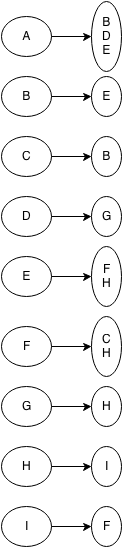
\includegraphics[scale=0.5]{images/31_3.png}
	
	\item[4.] What adjacency lists represent the graph in Figure 30-18a of the previous chapter?
		
		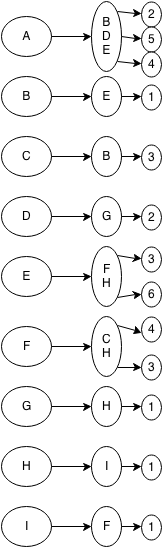
\includegraphics[scale=0.5]{images/31_4.png}
	
	\item[6.] Suppose that you want only to test whether an edge exists between two particular vertices. Does an adjacency matrix or an adjacency list provide a more efficient way of doing this?
		
		\vspace{0.5cm}
		An adjacency matrix is more efficient because it takes $O(1)$ time to scan whether an edge exists between any two given vertices, while an adjacency list would take $O(n)$, where $n$ is the number of vertices.
		\vspace{0.5cm}
	
	\item[7.] Suppose that you want only to find all vertices that are adjacent to some particular vertex. Does an adjacency matrix or an adjacency list provide a more efficient way of doing this?
	
		\vspace{0.5cm}
		An adjacency list is more efficient because finding all the neighbors of a particular vertex only requires traversing the appropriate list, while an adjacency list would need to look through all of the possible edges that could be connected to a particular vertex (traverse an entire row). Both take $O(n)$ time, where $n$ is the number of vertices, but the running time of using an adjacency list may be substantially faster than using an adjacency matrix.
		\vspace{0.5cm}
	
	\item[17.] A \textbf{loop} is an edge that starts and ends at the same vertex. Figure 31-5 shows an example of a loop in a directed, weighted graph.
		\begin{enumerate}
			\item Give an example of a problem where allowing loops would be useful.
			
				\vspace{0.5cm}
				Mapping out the love emotion in a group of individuals. The vertices are people. The edges represent love between people. There will be people that love themselves and others, but some that do not. The people that love themselves, will have an edge from and to themselves.
				\vspace{0.5cm}
				
			\item Can the adjacency matrix and adjacency list representations of a graph support loops?
				
				\vspace{0.5cm}
				Both the adjacency matrix and adjacency list representations of a graph support loops. Adjacency matrices have the entries $a_{ij}$, where $i = j$ that can be used to represent loops for vertex $i$. Adjacency lists can just add an edge from one vertex to itself by adding that to the appropriate adjacency list.
		\end{enumerate}
\end{enumerate}

\end{document}